\documentclass{article}

% formatação do documento -----------------------------------------------------

% ajustar margem
\usepackage[top=3cm, bottom=3cm, left=3cm, right=3cm]{geometry}

% funcionar caracteres em português
\usepackage[utf8]{inputenc}
\usepackage[T1]{fontenc}
% \usepackage{hyphenat} 
\usepackage[portuguese]{babel}
\usepackage{adjustbox}
\usepackage{longtable}
\usepackage{pdflscape}
\usepackage{booktabs}
\usepackage{float}
% espaçamento duplo
\usepackage{setspace}
\onehalfspace 

% título e autores do artigo
\title{\textbf{Nowcasting Brasil}}

\author{
\textbf{Pedro G. Costa Ferreira} \\
\small{FGV IBRE}
\and
\textbf{Daiane Marcolino de Mattos}\\
\small{FGV IBRE}
\and
\textbf{Guilherme Branco Gomes}\\
\small{FGV EPGE}
\and
\textbf{Tiago dos Guaranys Martins}\\
\small{FGV EPGE}
}

\date{}

% permitir links e formatá-los
\usepackage{hyperref}
\hypersetup{colorlinks = true, linkcolor = purple, citecolor = purple, urlcolor = black}

% referências
\usepackage[round]{natbib}

% parágrafo
\usepackage{indentfirst}

% código verbatim
\usepackage{fancyvrb}
\fvset{formatcom=\singlespacing} % espaço simples

% múltiplas figuras
\usepackage{graphicx}
%\usepackage{caption}
\usepackage{subcaption}
\usepackage[font={footnotesize}]{caption}

% tabelas + nota em tabelas
\usepackage{booktabs}
\usepackage[flushleft]{threeparttable}

% operadores matemáticos
\usepackage{amsmath}
\usepackage{xfrac}

% editar cor do texto \textcolor{cor}{texto}
\usepackage{xcolor}

\usepackage{Sweave}
\begin{document}
\Sconcordance{concordance:Artigo.tex:Artigo.Rnw:%
1 70 1 1 0 402 1}


\maketitle % aparecer o título e o autor

\begin{abstract}
Inserir resumo aqui
\end{abstract}

Palavras-chave: nowcasting, PIB, dynamic factors model.

{\let\thefootnote\relax\footnotetext{Somos gratos a Domenico Giannone por disponibilizar os códigos em \textsf{Matlab}, assim como comentários relevantes sobre a bibliografia.}}


\section{Introdução}\label{intro}

Decisões de política monetária e investimento são tomadas com base nas condições presentes e futuras da economia mesmo quando as variáveis usadas para descrever esse estado não estão acessíveis. Esse é particularmente o caso do PIB do Brasil que é divulgado, em média, 60 dias após o trimestre de referência. Por conta disso, a previsão em tempo real, ou simplesmente \textit{nowcasting}, se torna um tema de relevância.




O termo \textit{nowcasting} é cunhado em \cite{giannoneetal2008} e definido como a previsão do
presente, do passado recente ou do futuro próximo. Duas outras terminologias também são utilizadas e ajudam a complementar a definição de previsões ao longo do tempo. A terminologia \textit{nowcasting} refere-se à previsão da variável durante o seu período de realização. A terminologia \textit{backcasting} refere-se à previsao da variável após o seu período de realização, porém esta ainda não foi observada/divulgada. E, por fim, a terminologia \textit{forecasting} refere-se à previsao da variável antes do seu período de realização. Para tornar mais claro o entendimento, suponha que se deseja obter a previsão do PIB para o 2º trimestre de 2017. Se o período corrente é uma data contida no 2º trimestre de 2017, então a previsão é classificada como nowcasting. No entanto, se a data atual é anterior ao 2º trimestre de 2017, diz-se forecasting. E por último, se a data atual é posterior ao 2º trimestre de 2017 e o PIB ainda não foi divulgado, então faz-se backcasting.

Os métodos de previsão em tempo real, que se desenvolveram nas últimas décadas, são baseados em modelos de fatores dinâmicos (DFM) e dependem de algum poder computacional para lidar com uma grande quantidade de dados. Veja \cite{stockwatson2006} para uma revisão a respeito dessa literatura. No artigo \cite{giannoneetal2008}, os autores mostram como reduzir em apenas dois fatores dinâmicos a informação contida em dezenas de séries temporais mensais com o intuito de explicar o PIB (dos Estados Unidos) de curto prazo dos trimestres cuja informação ainda não está disponível. Após esse estudo, muitos outros continuaram explorando o uso de DFM na previsão em tempo real, como por exemplo \cite{banburarunstler2011} e \cite{banburaetal2011}. No primeiro os autores fazem uma análise mostrando como a divulgação de certas variáveis influenciam na atualização da previsão do PIB. Além disso, os autores também propõem uma medida mensal para a variável trimestral, uma vez que os fatores extraídos são mensais. No segundo, os autores propõem estimar o modelo via outro método (Expectation-Maximization) e não mais por dois estágios como se fazia em \cite{giannoneetal2008}.

Nesse artigo tem-se o objetivo de encontrar um modelo de previsão para o PIB do Brasil segundo as propostas desenvolvidas nos artigos do parágrafo anterior. Para disseminar o uso da metodologia e reproduzir esse trabalho, desenvolveu-se o pacote \texttt{nowcasting} no \textsf{R} com tais métodos e algumas outras ferramentas que facilitam o tratamento de séries temporais para tal uso e que permitem analisar a importância de cada variável numa previsão. As funções de estimação foram apenas traduzidas para a linguagem, uma vez que \cite{giannoneetal2008} e \cite{banburaetal2011} forneceram os códigos em \textsf{Matlab}.

A estrutura do artigo é a seguinte: na seção \ref{metodo} é apresentadado brevemente o arcabouço teórico sobre modelos de fatores dinâmicos e também a base de dados; na seção \ref{nowcastingBR} tem-se os resultados da aplicação metodológica e a análise dos resultados. Por fim, na seção \ref{conclusao}, têm-se as considerações finais. Embora todo o contexto apresentado aqui seja referente ao PIB, a metodologia pode ser aplicada a outras séries temporais.

\section{Metodologia}\label{metodo}

\subsection{Modelo de Fatores Dinâmicos}\label{DFMmodel}

Seja $x_t = (x_{1,t},x_{2,t}, ..., x_{N,t})^{'}$ o vetor que representa as $N$ séries temporais mensais transformadas para satisfazerem a suposição de estacionariedade. A especificação geral do modelo de fator dinâmico (DFM em inglês) é dada por:

\begin{align}
x_t   &= \mu + \Lambda f_t + \varepsilon_t \label{eq_xt} \\
f_{t} &= \sum_{i=1}^{p} A_i f_{t-i} + B u_t, \quad u_t \sim NID(0,I_q) \label{eq_ft}
\end{align}

em que $\mu$ é o vetor de médias incondicionais, $f_t$ é o vetor de fatores comuns (não observados) de dimensão $r \times 1$ modelados por um processo VAR(p) em que as matrizes $A_i$ de dimensão $r \times r$ representam os coeficientes do processo autorregressivo, B é uma matriz de coeficientes de dimensão $r \times q$, $\Lambda$ é uma matriz de constantes de dimensão $N \times r$ e $\varepsilon_t$ é um vetor de componentes idiossincráticos, tal que $\Psi = E[\varepsilon_{t} \varepsilon^{'}_{t}]$. Assume-se ainda que $E[\varepsilon_t u_{t-k}'] = 0$ para qualquer $k$. %, que pode seguir um processo AR(q):

No chamado \textit{modelo de fatores dinâmicos exato} assume-se que os componentes de erro são mutualmente não correlacionados em todos os lags, isto é, $E[\varepsilon_{i,t} \varepsilon_{j,s}] = 0$ para $i \neq j$. No entanto, é possível que a componente idiossincrática siga um processo AR(p) tal como se mostra na equação (\ref{eq_arq}). Tal procedimento é encontrado com mais detalhes em \cite{banburaetal2011}.

\begin{equation}\label{eq_arq}
\varepsilon_{i,t} = \sum_{i=1}^{p} \alpha_i \varepsilon_{i,t-i} + e_{i,t}, \quad e_{i,t} \sim NID(0,\sigma^2_i)
\end{equation}

em que $E[e_{i,t} e_{j,s}] = 0$ para $i \neq j$.



Veja um exemplo da representação matricial da equação \ref{eq_ft} do modelo apresentado considerando as ordens $r = 2$, $p = 2$ e $q = 2$.


\begin{equation}
\begin{bmatrix}
f_{1,t}\\
f_{2,t}\\
f_{1,t-1}\\
f_{2,t-1}
\end{bmatrix}
=
\begin{bmatrix}
a^1_{1,1} & a^1_{1,2} & a^2_{1,1} & a^2_{1,2} \\
a^1_{2,1} & a^1_{2,2} & a^2_{2,1} & a^2_{2,2} \\
1 & 0 & 0 & 0 \\
0 & 1 & 0 & 0
\end{bmatrix}
\begin{bmatrix}
f_{1,t-1}\\
f_{2,t-1}\\
f_{1,t-2}\\
f_{2,t-2}
\end{bmatrix}
+
\begin{bmatrix}
b_{1,1} & b_{1,2}\\
b_{2,1} & b_{2,2}\\
0 & 0\\
0 & 0
\end{bmatrix}
\begin{bmatrix}
u_{1,t}\\
u_{2,t}
\end{bmatrix}
\end{equation}

%ou em forma matricial

% \[
\begin{equation}
F_t
=
\begin{bmatrix}
A_1 & A_2 \\
I_2 & 0
\end{bmatrix}
F_{t-1}
+
B
u_t
\end{equation}


\subsection{Variáveis trimestrais e mensais}\label{variaveisQM}

Para que a modelagem apresentada suporte frequências mensais e trimestrais, é utilizada a transformação proposta em \cite{marianomurasawa2003}. Assim é possível que variáveis trimestrais como PIB sejam explicadas por outras variáveis de frequências mensais (fatores) ao se obter representações trimestrais para a variável mensal.

Seja $Y_t^M$ o nível de uma variável mensal que representa o fluxo. A representação trimestral dessa variável $Y_t^Q$ é dada por:

\begin{equation}
Y_t^Q = Y_t^M + Y_{t-1}^M + Y_{t-2}^M, \quad  t = 3,6,9,...
\end{equation}

Defina $y_t = Y_t^M - Y_{t-1}^M$ e $y_t^Q = Y_t^Q - Y_{t-3}^Q$. Desse modo pode-se escrever $y_t^Q$ em função de $y_t$ de acordo com o seguinte filtro:

\begin{equation}
y_t^Q = y_t + 2y_{t-1} + 3y_{t-2} + 2y_{t-3} + y_{t-4}, \quad  t = 3,6,9,...
\end{equation}

Assim é possível transformar diferenças mensais em diferenças trimestrais. Além disso, se a variável de interesse for uma taxa de variação, é válida a aproximação a seguir:

\begin{equation}
log(y_t^Q) \approx log(y_t) + 2log(y_{t-1}) + 3log(y_{t-2}) + 2log(y_{t-3}) + log(y_{t-4})
\end{equation}

\subsection{Estimação}\label{estima}

O método de estimação utilizado nesse paper é definido como \textit{Two Stages}, em que as variáveis explicativas em $x_t$ são de mesma periodicidade (mensal) e a variável resposta de periodicidade trimestral. Essa abordagem é apresentada no trabalho seminal de \cite{giannoneetal2008}. 

Considerando o modelo de fatores dinâmicos exato, a estimação dos fatores dinâmicos é feita em duas etapas. No primeiro estágio, utilizando um painel ($\bar{X}_t$) balanceado e padronizado, são estimados os parâmetros das matrizes $\Lambda$ e $f_t$ via PCA (Principal Components Analysis). Por balanceado entende-se as variáveis em $x_t$ sem missings e outliers. A padronização é importante pois a estimação via PCA não é invariante a escala. Os estimadores $\hat\Lambda$ e $\hat{f}_t$ podem ser obtidos resolvendo o problema de otimização em (\ref{otimiza_ft}).

\begin{equation}\label{otimiza_ft}
\min_{f_1,...,f_T,\Lambda} \frac{1}{NT} \sum_{t=1}^T (\bar{X}_t -\Lambda f_t)'(\bar{X}_t -\Lambda f_t) \quad s.t. \quad N^{-1} \Lambda'\Lambda = I_r
\end{equation}

Em seguida, o estimador da matriz de variância e covariância de $\varepsilon_t$ é dado por

\begin{equation}
\hat{\Psi} = diag\Bigg(\frac{1}{T} \sum_{t=1}^T (\bar{X}_t -\hat{\Lambda} \hat{f}_t)(\bar{X}_t -\hat{\Lambda} \hat{f}_t)'\Bigg)
\end{equation}

De acordo com \cite{stockwatson2011}, a solução de (\ref{otimiza_ft}) é tal que $\hat{\Lambda}$ são os autovetores da matriz de variância e covariância de $\bar{X}_t$ associados aos $r$ maiores autovalores e $\hat{f_t}$ são as $r$ primeiras componentes principais de $\bar{X}_t$. Os coeficientes das matrizes $A_i$, $i = 1,2,...,p$, são estimados por OLS ao regredir $f_t$ em $f_{t-1},...,f_{t-p}$. Por fim $BB'$ é estimado como sendo a matriz de covariância dos resíduos dessa regressão.

No segundo estágio, utiliza-se \textit{Kalman smoothing} para reestimar os fatores para o painel não balanceado $x_t$ considerando os parâmetros obtidos na etapa anterior. Nesse contexto, duas opções podem ser consideradas ao estimar os fatores:

\begin{itemize}
\item \textit{quarterly factors}: as variáveis explicativas mensais podem ser transformadas para representarem quantidades trimestrais seguindo o procedimento visto na seção \ref{variaveisQM}. Portanto, os fatores embora mensais também representarão quantidades trimestrais e, consequentemente, poderão ser transformados em variáveis de periodicidade trimestral, e assim a equação (\ref{reg}) pode ser estimada para a previsão da variável resposta.

\item \textit{monthly factors}: outra opção é estimar os fatores sobre as variáveis originais e ao final aplicar a transformação vista na seção \ref{variaveisQM} aos fatores para que representem quantidades trimestrais. Em seguida cria-se a variável de periodicidade trimestral que será usada para a previsão da variável resposta em (\ref{reg}).
\end{itemize}

\begin{equation}\label{reg}
y_t = \beta_0 + \beta' \hat{f}_t  + e_t
\end{equation}

Os parâmetros da equação (\ref{reg}) são estimados por OLS e a previsão de $y_{t+h}$ é obtida como

\begin{equation}
\hat{y}_{t+h} = \hat{\beta_0} + \hat{\beta}' \hat{f}_{t+h}
\end{equation}



\subsection{Base de dados}\label{base}

As variáveis explicativas utilizadas na previsão do PIB do Brasil foram selecionadas com base nas opiniões de especialistas em previsões do PIB do Brasil e nos trabalhos desenvolvidos em \cite{giannoneetal2008} e em \cite{banburaetal2011}. Ao todo tem-se 130 variáveis e estas são apresentadas na Tabela \ref{tab:long} (Apêndice). Nessa tabela também mostra-se qual transformação aplicou-se a cada variável a fim de torná-las estacionárias. As tranformações são: 0: a série observada é preservada; 1: taxa de crescimento mensal; 2: diferença mensal; 3: diferença da taxa de crescimento interanual; 4: diferença da diferença anual. Além disso, mostra-se também o tempo em dias que cada variável demora para ser divulgada (\textit{delay}). Essa última informação é útil para a estimação das previsões para um período passado, permitindo a criação da base de dados supostamente observada em uma data específica.

A variável resposta que se deseja prever é o PIB do Brasil. A variável trimestral foi coletada sem ajuste sazonal e a transformação para estacionarizá-la é a 3 (diferença da taxa de crescimento interanual). Embora a variável prevista seja o nível, é de interesse dos analistas a previsão da variável em taxa de variação trimestral (contra o trimestre imediatamente anterior) e também em taxa de variação anual (contra o mesmo trimestre do ano anterior). Para obter a taxa de variação trimestral é necessário primeiramente remover a sazonalidade da variável em nível. O ajuste sazonal então foi realizado utilizando o software X-13ARIMA-SEATS seguindo a metodologia do IBGE\footnote{\url{ftp://ftp.ibge.gov.br/Contas_Nacionais/Contas_Nacionais_Trimestrais/Ajuste_Sazonal/X13_NasContasTrimestrais.pdf}}.  


\section{Real time do PIB brasileiro}\label{nowcastingBR}

Os resultados a seguir mostram o desempenho do modelo final seguindo a metodologia de fatores dinâmicos apresentada na seção \ref{metodo}. Para definir o modelo e alcançar um resultado desejável com um baixo erro de previsão, fez-se diferentes combinações com as diferentes quantidades \textit{r} de fatores dinâmicos, a ordem \textit{p} de defasagem dos fatores, o número \textit{q} de choques nos fatores e as duas opções de estimação para os fatores. A combinação escolhida foi a de p = 2, q = 2 e r = 2 com o método de estimação \textit{monthly factors} utilizando todas as variáveis descritas na Tabela \ref{tab:long} vista no apêndice.

As previsões que serão apresentadas ocorreram a cada sexta-feira de 7 de novembro de 2014 a 31 de dezembro de 2017  para o primeiro trimestre de 2015 até o quarto trimestre de 2017. Pode ser visto na tabela de erro de previsão Figura \ref{rmse39} que a cada semana que passa o erro de previsão diminui e percebe-se que quando estão prevendo o PIB do período que está dentro da amostra (nowcasting) vê-se que o erro cai ainda mais e fica próximo à 0.7.

\begin{figure}[H]
  \centering
  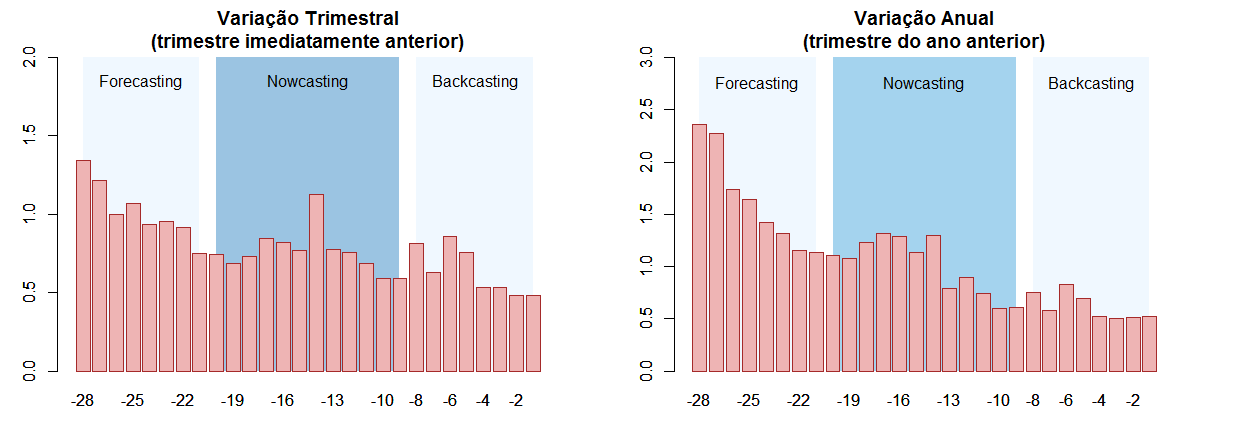
\includegraphics[width=1\textwidth]{rmse_nowcasting} % largura 13.11 altura 3.65
  \caption{RMSE das previsões do PIB do Brasil durante 39 semanas antes de sua divulgação}
  \label{rmse39}
\end{figure}

Como pode-se observar na figura \ref{Comparacao} vê-se que o erro de previsão é grande quando faltam 2 meses para começar o trimestre que está sendo previsto, porém com a divulgação de cada vez mais variáveis a cada semana percebe-se que quando se passa 1 mês dessa previsão ocorre um grande salto e o erro de previsão cai bruscamente. Como foi ressaltado no parágrafo anterior tem-se que o erro diminui mais a medida que se aproxima do começo do trimestre avaliado. 

Na figura \ref{Comparacao} vê-se a comparação do modelo em questão contra a previsão do boletim Focus, pode-se ver que o erro de previsão deles é muito pequeno comparado ao do modelo, porém quando entra no trimestre em questão, o erro se aproxima muito do erro do boletim Focus, visto que a PIB divulgado pelo IBGE seria a linha pontilhada como ressaltado na legenda da Figura \ref{Comparacao.

\begin{figure}[H]
  \centering
  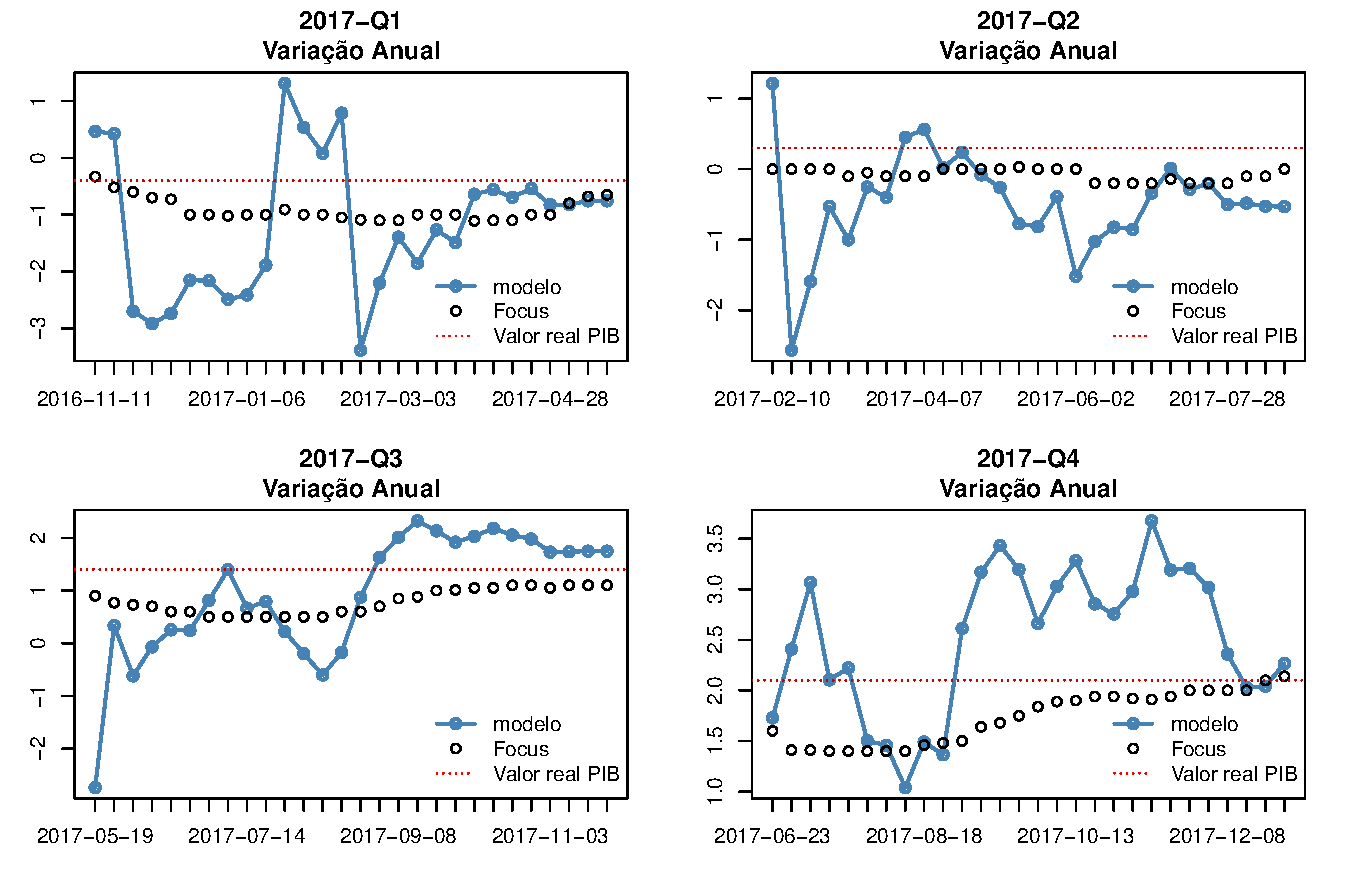
\includegraphics[width=1\textwidth]{ComparacaoFocusModelo} %largura 13.11 altura 3.65
  \caption{Comparação entre o nosso modelo e o Focus}
  \label{Comparacao}
\end{figure}

A figura \ref{fcst_variacoes} mostra o resultado do modelo prevendo o pib a cada trimestre (ponto vermelho), a variação da previsão até chegar na previsão final (linha vermelha) e o PIB que foi divulgado pelo IBGE (coluna azul).

\begin{figure}[H]
  \centering
  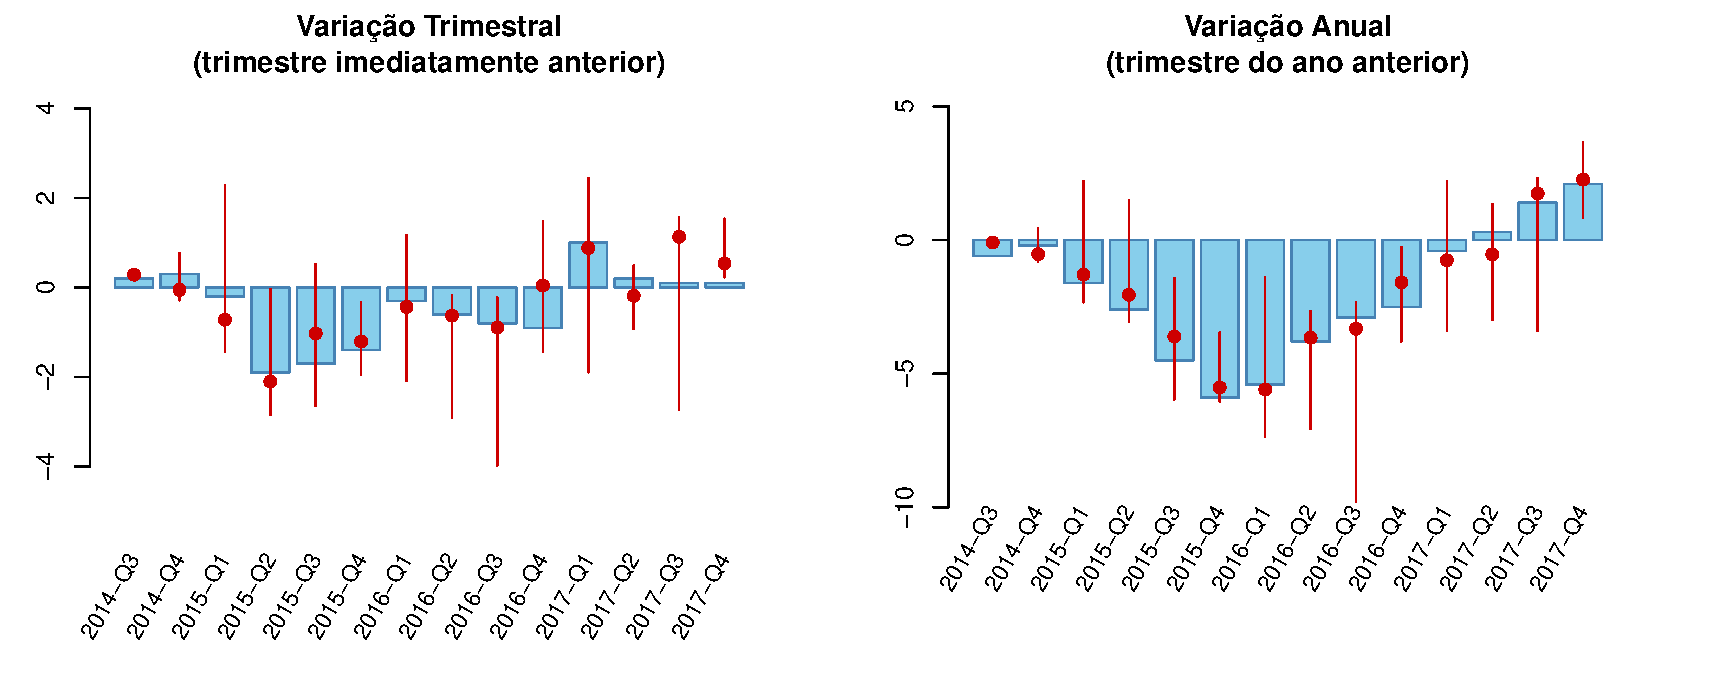
\includegraphics[width=1\textwidth]{fcst3anos_variacoes} % largura 13.11 altura 3.65
  \caption{Previsão do PIB do Brasil de 2014-Q1 a 2017-Q4}
  \label{fcst_variacoes}
\end{figure}


\textcolor{red}{mostrar link do shiny com a atualização da previsão atual, realtime}


\section{Considerações finais}\label{conclusao}

\textcolor{red}{concluir o trabalho e apresentar trabalhos futuros}

\bibliographystyle{apa-good}
\bibliography{refs}



\begin{landscape}
\section*{Apêndice}

\begin{center}
\begin{longtable}{|l|l|l|l|}

\caption{Variáveis explicativas}\label{tab:long} \\

\hline \multicolumn{1}{|c|}{\textbf{Series code}} & \multicolumn{1}{c|}{\textbf{Series name}} & \multicolumn{1}{c|}{\textbf{Transformation}} & \multicolumn{1}{c|}{\textbf{Delay}} \\ \hline
\endfirsthead

\multicolumn{3}{c}%
{{\bfseries \tablename\ \thetable{} -- continuação da página anterior}} \\
 % <<<<<<< HEAD
\hline \multicolumn{1}{|c|}{\textbf{Series code}} & \multicolumn{1}{c|}{\textbf{Series name}} & \multicolumn{1}{c|}{\textbf{Transformation}} & \multicolumn{1}{c|}{\textbf{Delay}} \\ \hline
 % =======
% >>>>>>> e8977d353c1435645224b462bf46129a5e4e5501
\endhead

\hline %\multicolumn{3}{|r|}{{Continued on next page}} \\ \hline
\endfoot

\hline \hline
\endlastfoot

serie1 & Exchange rate- Free- United States dollar (sale)-1 u.m.c/US\$ & 1 & 0 \\
serie12 & Interest rate- CDI & 1 & 0 \\
serie188 & National Consumer Price Index (INPC) & 4 & 14 \\
serie189 & General Price Index-Market (IGP-M) & 0 & 0 \\
serie192 & National Index of Building Costs (INCC) & 4 & 0 \\
serie193 & Consumer Price Index- Sao Paulo (IPC-FIPE) & 4 & 7 \\
serie194 & Cost of Living Index (ICV-Dieese) & 4 & 7 \\
serie206 & Staple food basket u.m.c & 1 & 7 \\
serie225 & Wholesale Price Index (IPA) & 0 & 14 \\
serie432 & Interest rate- Selic target & 1 & 0 \\
serie433 & Broad National Consumer Price Index (IPCA) & 4 & 7 \\
serie1178 & Interest rate- Selic in annual terms (basis 252) & 4 & 0 \\
serie1344 & Installed capacity utilization- General(FGV) & 3 & 0 \\
serie1373 & Vehicle production (total) & 3 & 14 \\
serie1374 & Passenger cars and light commercial vehicles production & 3 & 14 \\
serie1375 & Truck production & 3 & 14 \\
serie1376 & Bus production & 3 & 14 \\
serie1377 & Motorcycle production & 3 & 14 \\
serie1378 & Vehicle sales (total) & 3 & 14 \\
serie1379 & Domestic vehicle sales & 3 & 14 \\
serie1380 & Vehicle exports & 3 & 14 \\
serie1382 & Productions of mechanised cultivators & 4 & 14 \\
serie1383 & Four wheel tractor production & 3 & 14 \\
serie1384 & Track driven tractor production & 3 & 14 \\
serie1385 & Production of combined harvesters & 3 & 14 \\
serie1386 & Production of mechanical diggers & 3 & 14 \\
serie1387 & Other agricultural machinery & 3 & 14 \\
serie1388 & Production of agricultural machinery (total) & 3 & 14 \\
serie1389 & Petroleum derivatives production- crude oil & 1 & 42 \\
serie1390 & Petroleum derivatives production- LGN & 1 & 42 \\
serie1391 & Petroleum derivatives production- total & 1 & 42 \\
serie1392 & Petroleum derivatives production- natural gas & 1 & 42 \\
serie1402 & Electric energy consumption- Brazil- commercial & 3 & 42 \\
serie1403 & Electric energy consumption- Brazil- residential & 3 & 42 \\
serie1404 & Eletric energy consumption- Brazil- industrial & 3 & 42 \\
serie1405 & Eletric energy consumption- Brazil- other & 3 & 42 \\
serie1406 & Eletric energy consumption- Brazil- total & 3 & 42 \\
serie1453 & Credit sales Index & 3 & 21 \\
serie1454 & Cash Sales Index & 3 & 21 \\
serie1455 & Sales volume index in the retail sector- Total- Brazil & 3 & 70 \\
serie1483 & Sales volume index in the retail sector- Fuel and lubricants- Brazil & 3 & 70 \\
serie1496 & Sales volume index in the retail sector- Hypermarkets, supermarket, food, beverages and tobacco- Brazil & 3 & 70 \\
serie1522 & Sales volume index in the retail sector- Furniture and white goods- Brazil & 3 & 70 \\
serie1509 & Sales volume index in the retail sector- Textiles, Clothing and Footwear- Brazil & 3 & 70 \\
serie1548 & Sales volume index in the retail sector- Vehicles and motorcycles, spare parts- Brazil & 3 & 70 \\
serie1561 & Sales volume index in the retail sector- Hypermarkets, supermarket- Brazil & 3 & 70 \\
serie2053 & Net public debt- Balances in c.m.u. (million) - Total- Federal Government and Banco Central & 1 & 35 \\
serie2057 & Net public debt- Balances in c.m.u. (million) - Total- State governments & 1 & 35 \\
serie2058 & Net public debt- Balances in c.m.u. (million) - Total- Municipal governments & 1 & 35 \\
serie4393 & Consumer confidence index & 3 & 14 \\
serie4394 & Current economic conditions index & 3 & 14 \\
serie4395 & Future expectations index & 1 & 14 \\
serie4503 & Net public debt (\%GDP)- total- Federal Government and Banco Central & 2 & 35 \\
serie4506 & Net public debt (\% GDP)- Total- State and municipal governments & 2 & 35 \\
serie4507 & Net public debt (\%GDP)- total- State governments & 2 & 35 \\
serie4508 & Net public debt (\% GDP)- total- Municipal governments & 2 & 35 \\
serie4509 & Net public debt (\%GDP)- total- State enterprises & 2 & 35 \\
serie4513 & Net public debt(\%GDP)- total- consolidated public sector & 2 & 35 \\
serie7341 & Business confidence index- General & 1 & 0 \\
serie7357 & Steel production (1992= 100) & 3 & 42 \\
serie7384 & Sales of factory authorized vehicle outlets- Passenger cars sales & 3 & 7 \\
serie7385 & Sales of factory authorized vehicle outlets- Light commercial cars sales & 3 & 7 \\
serie7386 & Sales of factory authorized vehicle outlets- Truck sales & 3 & 7 \\
serie7412 & Balanced checks - in 1000 & 3 & 98 \\
serie7413 & Returned checks - in 1000 & 3 & 98 \\
serie7415 & BNDES system disbursements- Total & 3 & 21 \\
serie7416 & BNDES system disbursements- Manufacturing industry & 3 & 21 \\
serie7417 & BNDES system disbursements- Commerce and Services & 3 & 21 \\
serie7418 & BNDES system disbursements- Agricultural sector & 3 & 21 \\
serie7419 & BNDES system disbursements- Vegetable extraction & 3 & 21 \\
serie7478 & National consumer Price Index- Extended 15 (IPCA-15) & 0 & 0 \\
serie7495 & SINAPI & 0 & 14 \\
serie7832 & Ibovespa- monthly percent change & 0 & 14 \\
serie13667 & Percent of 90 days past due loans of financial institutions under public control - Total & 1 & 14 \\
serie13673 & Percent of 90 days past due loans of financial institutions under national private control - Total & 1 & 14 \\
serie13679 & Percent of 90 days past due loans of financial institutions under foreign control - Total & 1 & 14 \\
serie13685 & Percent of 90 days past due loans of financial institutions under private control - Total & 1 & 14 \\
serie20048 & Commodity Index - Brazil (until Nov/2017) & 1 & 14 \\
serie20050 & Commodity Index - Brazil Agriculture (until Nov/2017) & 1 & 14 \\
serie20051 & Commodity Index - Brazil metal (until Nov/2017) & 1 & 14 \\
serie20052 & Commodity Index - Brazil Energy (until Nov/2017) & 1 & 14 \\
serie20099 & Pharmac., medical, orthop, and perfumery articles & 3 & 70 \\
serie20101 & Books, newspaper, megazines & 3 & 70 \\
serie20102 & Office, comp./ comunic, equip & 3 & 70 \\
serie20104 & Other art. Of personal use & 3 & 70 \\
serie20105 & Building materials & 3 & 70 \\
serie20106 & Broad trade sector & 3 & 70 \\
serie20339 & Sondagem de serviços - Índice de Confiança de Serviços- Dessazonalizado & 1 & 7 \\
serie20340 & Sondagem de Serviços - Índice de Expectativas (IE-S) - Dessazonalizado & 1 & 7 \\
serie20341 & Residential Real Estate Collateral Value Index & 1 & 98 \\
serie21637 & PMS- Nominal revenue from services - Total - Brazil & 3 & 42 \\
serie21859 & General (2012=100) & 3 & 35 \\
serie21861 & Physical Production- Mineral extraction & 3 & 35 \\
serie21862 & Physical Production - Manufacturing Industry & 3 & 35 \\
serie21863 & Physical Production - Capital goods & 3 & 35 \\
serie21864 & Physical Production- Intermediate goods & 3 & 35 \\
serie21865 & Physical Production - Consumer goods & 3 & 35 \\
serie21866 & Physical Production - Durable goods & 3 & 35 \\
serie21867 & Physical Production - Semi durable and nondurable goods & 3 & 35 \\
serie21868 & Physical Production - Production of construction inputs & 3 & 35 \\
serie21924 & Industrial Production (2012=100)- Southeast Region & 3 & 35 \\
serie21930 & Industrial Production (2012=100)- Northern Region & 3 & 35 \\
serie21934 & Industrial Production (2012=100)- South & 3 & 35 \\
serie21939 & Industrial Production (2012=100)- Central- Western Region & 3 & 35 \\
serie21961 & Industrial Production (2012=100)- Northeast & 3 & 35 \\
serie22704 & Balance on goods and services - monthly - net & 3 & 21 \\
serie22705 & Balance on goods and services - monthly - credit & 3 & 21 \\
serie22706 & Balance on goods and services - monthly - debit & 3 & 21 \\
serie22707 & Balance on goods- Balance of Payments - monthly- net & 3 & 21 \\
serie24352 & Capacity utilization- manufacturing industry (FGV) & 1 & 21 \\
serie24369 & Enemployment - PNAD & 3 & 28 \\
serie24370 & Working age populaton - Continuous PNAD & 1 & 28 \\
serie24378 & Labor force population - Continuous PNAD & 1 & 28 \\
serie24379 & Employed population - Continuous PNAD & 3 & 28 \\
serie24382 & Real habitually average earnings of employed people- Continuous PNAD & 1 & 28 \\
serie25241 & Registered employees Index - Manufacturing & 3 & 28 \\
ICI & ICI with seasonal adjust - Industry confidence index & 1 & 0 \\
ISA & ISA with seasonal adjust - Industry confidence index - Actual situation & 1 & 0 \\
IE & IE with seasonal adjust - Industry confidence index - Expectation & 1 & 0 \\
ICOM & ICOM with seasonal adjust-Retail sector extended index & 1 & 0 \\
ISACOM & ISA-COM with seasonal adjust-Retail sector extended actual situtation index & 1 & 0 \\
IECOM & IE-COM with seasonal adjust-Retail sector extended expected index & 1 & 0 \\
ICS & ICS with seasonal adjust - Service confidence index & 1 & 0 \\
ISAS & ISA-S with seasonal adjust - Service confidence index- Actual situation & 1 & 0 \\
IES & IE-S with seasonal adjust - Service confidence index- Expectiation & 1 & 0 \\
IAEAGRO & Economy agriculture activities & 3 & 8 \\
IAEIND & Economy industrial activities & 3 & 8 \\
IAESERV & Economy services activities & 3 & 8 \\
IAEIMP & Economy taxes activities & 3 & 8 \\
IAE & Economy activities & 3 & 8 \\



\end{longtable}
\end{center}
\end{landscape}

\end{document}
